\documentclass[sans]{beamer}

% \usetheme{Boadilla}
\mode<presentation>
{
	% \usetheme{CambridgeUS}
	\usetheme{Hannover}
	% \usetheme{Bergen}
	\usecolortheme{whale}
	% \usefonttheme{serif}
	% \usefonttheme{professionalfonts}
	% \usefonttheme{structureitalicserif}
}

\usepackage{cmap}
\usepackage{listings}
\usepackage{lmodern}
\usepackage{color}
\usepackage{minted}
\usepackage{graphicx}
\usepackage{tikz}
\usepackage{wrapfig}

% \usepackage[labelformat=empty]{subcaption}
\usepackage[labelformat=empty]{caption}

% \usefonttheme{professionalfonts} % using non standard fonts for beamer
% \usefonttheme{sansserif} % default family is serif
% \usepackage{fontspec}
% \usepackage[T2A]{fontenc}
% \setmainfont{Comic Sans MS}

% \usepackage[utf8]{inputenc}
% \usepackage[russian]{babel}

\usepackage{fontspec}
% \setmainfont[Mapping=tex-text]{CMU Serif}



\usepackage{polyglossia}
\setdefaultlanguage{russian}

% \newfontfamily\cyrillicfont[Script=Cyrillic]{Comic Sans MS}
% \newfontfamily{\cyrillicfontt} {Comic Sans MS}
% \newfontfamily{\cyrillicfonttt}{Comic Sans MS}

\setmainfont[Ligatures=TeX]{DejaVu Serif}
\setsansfont[Ligatures=TeX]{DejaVu Sans}
% \setmainfont[Ligatures=TeX]{Comic Sans MS}
% \setsansfont[Ligatures=TeX]{Comic Sans MS}
\setmonofont{DejaVu Sans Mono}

% \setmathfont{XITS Math}
% \defaultfontfeatures{Scale=MatchLowercase,Mapping=tex-text}

\begin{document}

\title[РФС]{Распределенные ФС}

\institute{СП, СПбГУ}

\author
[Подкопаев Антон]{Подкопаев Антон, \texttt podkoav239@gmail.com}
\date [07-10-13]{14 октября 2013}



\begin{frame}[plain]
	\titlepage
	% По мотивам лекции Д.Барашева в CSCenter
\end{frame}

\section{Основные концепции}

\begin{frame}{Файловая система}
	\begin{itemize}
		\item Модель данных, программные компоненты, персистентные структуры данных и API
		\item Абстракция для доступа к данным, находящимся на физическом носителе
		\item Традиционная модель
		\begin{itemize}
			\item Файл --- объект с именем и некоторым содержанием
			\item Каталог --- список файлов и подкаталогов
			\item Каталоги и файлы --- пространство имен
			\item Файл уникально идентифицируется путем
		\end{itemize}
	\end{itemize}
\end{frame}

\begin{frame}{Метаинформация}
	Для ФС важна метаинформация --- название файла, список блоков, время модификации, права доступа 
\end{frame}

\begin{frame}{Локальные ФС}
	\begin{itemize}
		\item Некоторая интеграция с ядром ОС
		\item Данные на локальном HDD
		\item Блоки размером в несколько килобайт
		\item Кеширование страниц
	\end{itemize}
\end{frame}

\section {Особенности РФС}

\begin{frame}{Распределенная ФС}
	\begin{itemize}
		\item Компоненты распределены по разным машинам
		\item Распределенность существенно влияет на принимаемые решения
	\end{itemize}
	\hfill
	{\it Ваш К.О.}
\end{frame}

\begin{frame}{Компоненты РФС}
	\begin{itemize}
		\item {\color{red} Клиент}
		\begin{itemize}
			\item API прикладных приложений и код для коммуникации с сервером
		\end{itemize}

		\item {\color{red} Сервер данных}

		\begin{itemize}
			\item Содержимое файлов
		\end{itemize}

		\item {\color{red} Сервер метаданных}

		\begin{itemize}
			\item Информация о местоположении файла и еще кое-что
		\end{itemize}
	\end{itemize}
\end{frame}

\begin{frame}{Аспекты функционирования}
	\begin{itemize}
		\item Прозрачность размещения файлов
		\item Совместный доступ
		\item Кеширование
		\item Репликация
		\item Масштабируемость
	\end{itemize}
\end{frame}

\begin{frame}{Прозрачность размещения файлов}
	\begin{itemize}
		\item Прикладному ПО известен только путь
		\item Чем меньше информации о физическом местоположении, тем лучше
	\end{itemize}
\end{frame}

\begin{frame}{Совместный доступ и кеширование}
	\begin{itemize}
		\item Централизованная ФС
		\begin{itemize}
			\item Атомарные чтения и запись, блокировки, журналирование
		\end{itemize}
		\item Распределенная ФС
		\begin{itemize}
			\item Сетевые задержки, репликация усложняет жизнь
		\end{itemize}
	\end{itemize}
\end{frame}

\begin{frame}{Варианты управления СД}
	\begin{itemize}
		\item Синхронные чтение/запись
		\item Write-through cache
		\item Файлы неизменяемые после создания
		\item Append-only
		\item Уведомление о изменениях для клиентов, открывших файл
		\item Полноценные транзакции
	\end{itemize}
\end{frame}

\begin{frame}{Репликация}
	\begin{itemize}
		\item Синхронная и асинхронная
		\item Политика согласованности реплик
		\item Запись в реплики
	\end{itemize}
\end{frame}

\begin{frame}{Масштабируемость}
	\begin{itemize}
		\item Стремимся к линейной
			\begin{itemize}
				\item было {\color{blue} N} дисков и {\color{magenta} K} машин
				\item стало на {\color{blue} 2N} данных --- добавили {\color{blue} N} дисков, сохранили пропускную способность
				\item добавили {\color{magenta} K} машин --- получили в два раза большую пропускную способность
			\end{itemize}
		\item На практике есть препятствия
		\begin{itemize}
			\item пропускная способность сети, сетевых интерфейсов серверов, производительсность сервера метаданных, блокировки
		\end{itemize}
	\end{itemize}
\end{frame}

% TODO: мб все-таки добавить пару слов про историю, см вики

\section{Обзор}

\subsection{NFS}

\begin{frame}{NFS}
	NFS у всех на слуху...
\end{frame}

\begin{frame}{NFS}
	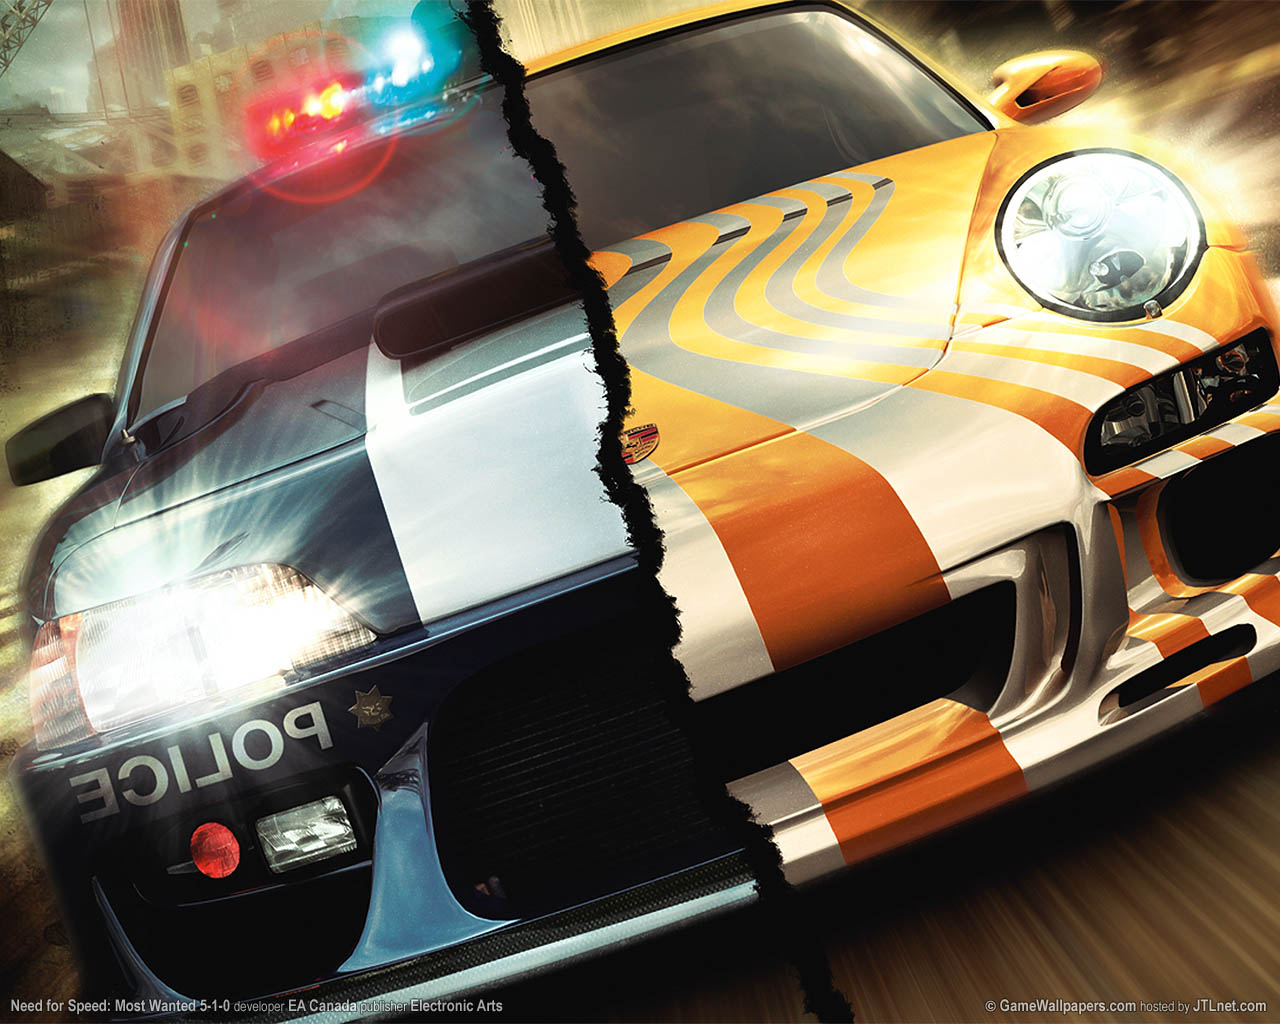
\includegraphics[width = \linewidth]{images/nfs.png}
\end{frame}

\begin{frame}{NFS}
	\begin{itemize}
		\item Network File System
		\item Sun, 1984
		\item POSIX API
		\item На сервере NFS работает с интерфейсом файловой системы
		\item Поддержка блокировок и сессионного кеширования
	\end{itemize}
\end{frame}

\begin{frame}{NFS. Устройство}
	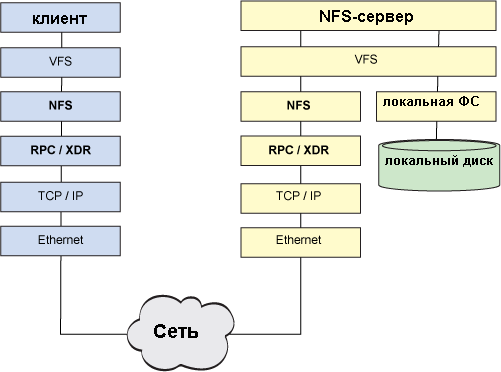
\includegraphics[width = \linewidth]{images/nfsScheme.png}
\end{frame}

\subsection{AFS}

\begin{frame}{AFS}
	\begin{itemize}
		\item Andrew File System
		\item Carnegie Mellon, 1980-е
		\item Сессионое кеширование, нотификации об изменениях, блокировки файлов
		\item Моментальные read-only снимки томов
		\item Не POSIX API
	\end{itemize}
\end{frame}

\subsection{CIFS}

\begin{frame}{CIFS}
	\begin{itemize}
		\item Common Internet File System
		\item ...aka SMB
		\begin{itemize}
			\item Server Message Block
			\item Samba
		\end{itemize}
		\item ...aka Windows Shared Folders
		\item IBM, 1983
		\item Microsoft, 1996
		\item Уступающие блокировки, блокировки файлов
		\item Аутентификация коллективного доступа
		\item Уведомление об изменении каталога
	\end{itemize}
\end{frame}

\begin{frame}{CIFS. Устройство}
	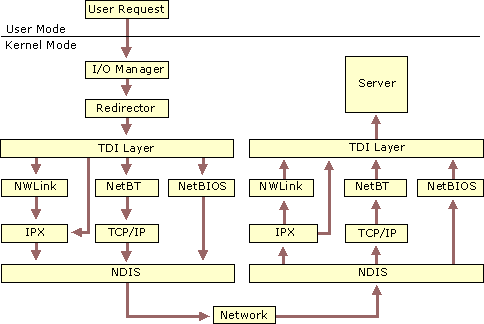
\includegraphics[width = \linewidth]{images/cifs.png}
\end{frame}

\subsection{GFS}

\begin{frame}{GFS}
	\begin{itemize}
		\item Google File System
		\item Начало 2000-ых

		\begin{block}{Предпосылки}
			\begin{itemize}
				\item Большие файлы (N Gb) записываются и читаются пакетными процессами (creawler, indexer)
				\item Пропускная способность важнее случайного доступа
				\item Ширпотребные компьютеры
			\end{itemize}
		\end{block}
	\end{itemize}
\end{frame}

\begin{frame}{Концепции архитектуры}
	\begin{itemize}
		\item Много файловых серверов, один активный сервер метаданных (мастер)
		\item Файлы хранятся фрагментами по 64 Mb
		\item Три реплики каждого фрагмента на различных файловых серверах
		\item Приоритетные операции с файлом
		\begin{itemize}
			\item Большое последовательное чтение
			\item Конкурентное наращивание
		\end{itemize}
		\item Кеширование на клиенте не производится
		\item Не POSIX API
	\end{itemize}
\end{frame}

\begin{frame}{Развертывание GFS}
	\begin{itemize}
		\item Ячейка --- единица развертывания
		\item В ячейке один мастер и много файловых серверов
		\item Ячейка GFS соответствует физическому датацентру
	\end{itemize}
\end{frame}

\begin{frame}{Взаимодействие клиена и мастера при чтении}
	\begin{itemize}
		\item Приложение собирается прочитать фрагмент
		\item GFS библиотека звонит мастеру, тот возвращает адреса
		{\color{blue} реплик} --- файловых серверов, хранящих фрагмент
		\item GFS библиотека напрямую звонит одному из файловых серверов
		с просьбой вернуть нужный диапазон внутри данного фрагмента
		\item Дальше прямое общение клиента и файлового сервера
	\end{itemize}
\end{frame}

\begin{frame}{Требования меняются}
	\begin{itemize}
		\item Google 2010-х годов --- интерактивные приложения
		\item Файлы меньше в размерах и больше в количестве
		\item Требование во времени произвольного доступа жестче
	\end{itemize}
	\pause
	{\color{blue}
		GFS в Google больше не используется, на смену пришел Colossus
	}
\end{frame}

\begin{frame}{Реализации, похожие на GFS}
	\begin{itemize}
		\item Реализация Google File System закрыта
		\item Открытые проекты с аналогичной архитектурой
		\begin{itemize}
			\item Apache HDFS: реализация на Java из проекта Hadoop
			\item QFS: реализация на C++
		\end{itemize}
	\end{itemize}
\end{frame}

\section{GlusterFS}

\begin{frame}{GlusterFS}
	\begin{itemize}
		\item OpenSource
		\item Сервер данных в том числе выполняет и функции сервера метаданных
	\end{itemize}

\end{frame}

\begin{frame}{Термины}
	\begin{itemize}
		% \item Brick     % The brick is the storage filesystem that has been assigned to a volume.
		% \item Subvolume % A brick after being processed by at least one translator.
		% \item Volume    % The final share after it passes through all the translators.

		\item Brick           % The brick is the storage filesystem that has been assigned to a volume.
		\item Логический диск % The final share after it passes through all the translators.

		%\item Client
		% The machine which mounts the volume (this may also be a server).
		%\item Server
		% The machine (virtual or bare metal) which hosts the actual filesystem in which data will be stored.

		% \item Translator
		% The brick's first translator (or last, depending on what direction data is flowing) is the storage/posix translator that manages the direct filesystem interface for the rest of the translators.
		% The configuration of translators (since GlusterFS 3.1) is managed through the gluster command line interface (cli), so you don't need to know in what order to graph the translators together.
		% All the translators hooked together to perform a function is called a graph. 		

		% \item Trusted storage pool
		\item Доверенные хранилища
		% Before you can configure a GlusterFS volume, you must create a trusted storage pool consisting of the
		% storage servers that provides bricks to a volume.
		% A storage pool is a trusted network of storage servers. 
	\end{itemize}
\end{frame}

\begin{frame}{Типы логических дисков}
	\begin{itemize}
		\item Распределеные
		\item Реплицируемые
		\item Разделяющие
		\vspace{1cm}
		\item Распределенные разделяющие
		\item Распределенные реплицируемые
		\item Разделяющие реплицируемые
	\end{itemize}
\end{frame}

\begin{frame}{Распределенные логические диски (1)}
	\begin{figure}[h]
		\centering
		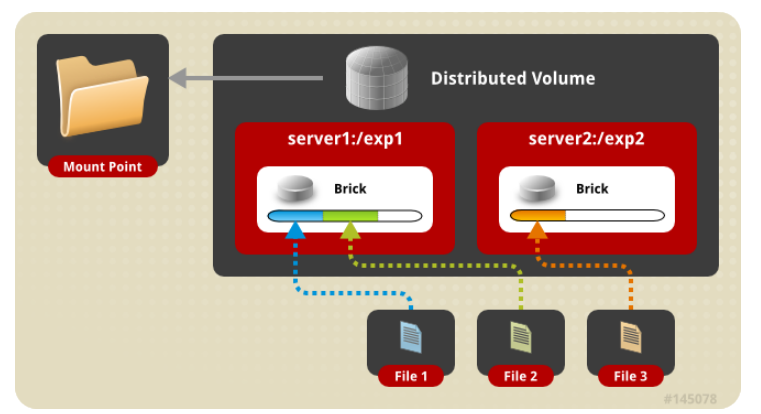
\includegraphics[width=0.8\linewidth]{images/distributed.png}
	\end{figure}
	% \begin{block}{}
		% gluster volume create test-volume server1:/exp1 server2:/exp2
	% \end{block}

	% The server that the files are written to is calculated by hashing the filename.
	% If the filename changes, a pointer file is written to the server that the new hash
	% code would point to, telling the distribute translator which server the file is actually on.
\end{frame}

\begin{frame}{Распределенные логические диски (2)}
	\begin{block}{Плюсы}
		\begin{itemize}
			% \item More servers - better scaling
			\item Больше серверов => выше производительность при параллельном доступе
			% in terms of random file access. As long as clients aren't all retrieving the same file,
			% their access should be spread pretty evenly across all the servers.

			% \item Increasing volume - adding a new server % on-the-fly
			\item Увеличение диска = добавление сервера (можно во время работы) % on-the-fly
		\end{itemize}
	\end{block}
	\begin{block}{Минусы}
		\begin{itemize}
			\item Потеря сервера = потеря данных на нем
			\item Файл не может быть больше размера узла
			\item Смена имени файла => дополнительное время на lookup
		\end{itemize}
	\end{block}
\end{frame}

\begin{frame}{Реплицируемые логические диски}
	\begin{figure}[h]
		\centering
		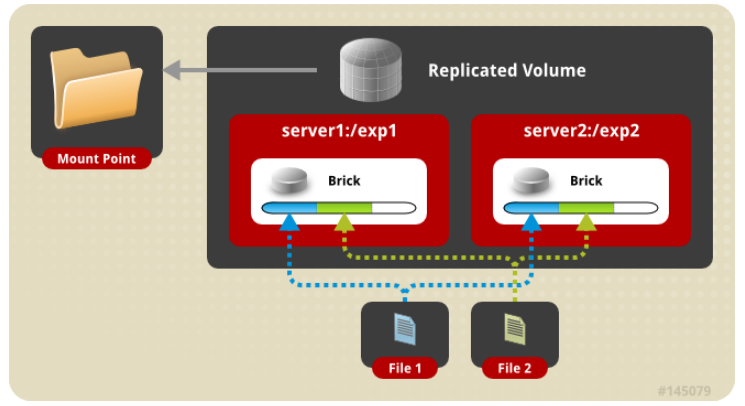
\includegraphics[width=0.8\linewidth]{images/replicated.png}
	\end{figure}
	% \begin{block}{}
	% 	gluster volume create test-volume replica 2 server1:/exp1 server2:/exp2
	% \end{block}
\end{frame}

\begin{frame}{Разделяющие логические диски}
	\begin{figure}[h]
		\centering
		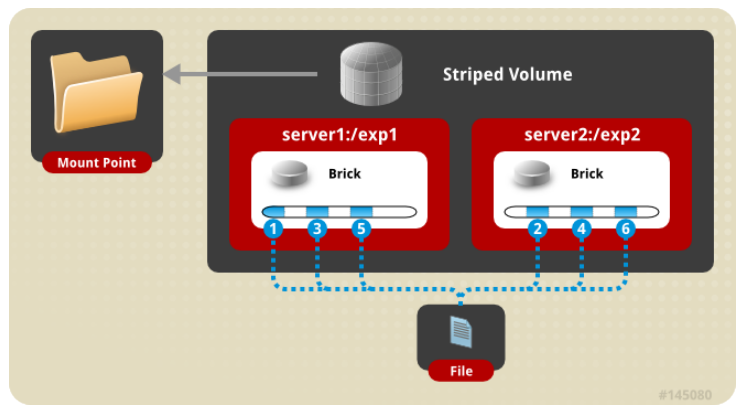
\includegraphics[width=0.8\linewidth]{images/striped.png}
	\end{figure}
	% \begin{block}{}
	% 	gluster volume create test-volume stripe 2 server1:/exp1 server2:/exp2
	% \end{block}
\end{frame}

\begin{frame}{Запуск GlusterFS (1)}
\footnotesize
	\begin{block}{}
		apt-get install glusterfs-server\\
		service glusterfs-server start\\
		service glusterfs-server status\\
	\end{block}
	\pause
	\begin{block}{}
		mkfs.xfs disk-image\\
		mount disk-image gluster\_disk\\
	\end{block}
	\pause
	\begin{block}{}
		gluster peer probe 192.168.1.105\\
		\vspace{0.2cm}
		gluster volume create gv0 replica 2\\
		            192.168.1.114:/home/us1/gluster\_disk\\
		            192.168.1.105:/home/us2/gluster\_disk\\

		\vspace{0.2cm}
		gluster volume start gv0\\
		gluster volume info\\

		mount -t glusterfs 192.168.1.105:/gv1 /mnt
	\end{block}
\end{frame}

\begin{frame}{Запуск GlusterFS (2)}
	\begin{block}{Распределенные}
		 gluster volume create test-volume server1:/exp1 server2:/exp2
	\end{block}
	\begin{block}{Реплицируемые}
		 gluster volume create test-volume replica 2 server1:/exp1 server2:/exp2
	\end{block}
	\begin{block}{Разделяющие}
		 gluster volume create test-volume stripe 2 server1:/exp1 server2:/exp2
	\end{block}
\end{frame}

\begin{frame}{Добавление серверов}
	\begin{block}{} 
		 gluster peer probe new\_server

		\pause
		 gluster volume add-brick vol\_name new\_brick

		\pause
		 gluster volume info
	\end{block}
	\pause
	\vspace{1cm}
	Для расширения реплицируемых (разделяющих) дисков надо добавлять количество серверов, кратное фактору реплики (разбиения)
\end{frame}

\begin{frame}{Удаление серверов}
	\begin{block}{} 
		 gluster volume remove-brick vol\_name new\_brick start

		\pause
		 gluster volume remove-brick vol\_name new\_brick status

		\pause
		 gluster volume remove-brick vol\_name new\_brick commit
	\end{block}
\end{frame}

\end{document}